\documentclass[10pt,a4paper]{article}
\usepackage[T1]{fontenc}
\usepackage[utf8]{inputenc}
\usepackage{lmodern}
\usepackage[margin=22mm,headheight=14pt]{geometry}
\usepackage{amsmath,amssymb,booktabs,tabularx,graphicx,caption,subcaption}
\usepackage{microtype,xcolor,fancyhdr,pdflscape,enumitem}
\usepackage[hidelinks,unicode]{hyperref}
\usepackage{xurl}
\definecolor{ink}{HTML}{18334A}
\definecolor{accent}{HTML}{246B83}
\hypersetup{pdftitle={Inferring Hidden Pokemon Builds from Competitive Team Data},pdfauthor={Pokemon Champions Assistant project},pdfsubject={M3.5.2 midterm research report, October 2026}}
\pagestyle{fancy}\fancyhf{}
\fancyhead[L]{\small\color{ink}Pok\'emon Champions Assistant}
\fancyhead[R]{\small Midterm research report}
\fancyfoot[L]{\footnotesize October 2026\quad\textbar\quad Research snapshot through M3.5.1}
\fancyfoot[R]{\thepage}
\setlength{\parindent}{0pt}\setlength{\parskip}{5pt}
\setlength{\emergencystretch}{1.5em}
\captionsetup{font=small,labelfont=bf,labelsep=period}
\setlist{nosep,leftmargin=*}
\setcounter{tocdepth}{1}
\newcommand{\SP}{\mathrm{SP}}
\newcommand{\E}{\mathcal{E}}
\newcommand{\F}{\mathcal{F}}
\newcommand{\figone}[3]{\begin{figure}[!ht]\centering\includegraphics[width=#2\linewidth]{figures/#1}\caption{#3}\end{figure}}
\newcommand{\boxkey}{Boxes show the interquartile range; orange lines mark medians and green triangles mark means. Whiskers reach the most extreme observations within 1.5 interquartile ranges of the box; circles are observations outside those limits. They are descriptive outliers, not erroneous records.}
\newcommand{\projkey}{Axes are positive classical-MDS projection coordinates, not individual SP stats. Color denotes the saved cluster index and black crosses denote observed medoids. Non-Euclidean dissimilarities cannot be reproduced exactly in two dimensions; negative eigenvalues and retained positive eigenmass are reported in the panels.}
% Generated only from preserved M3.5.1 numerical results.
\newcommand{\CandidateTable}{%
\begin{tabular}{llrrrl}\toprule Species & Model & $K$ & Sizes & Silhouette & Subsample ARI\\\midrule
Hatterene & learned & 1 & 13 & --- & 1.000/1.000/1.000\\
Hatterene & learned & 2 & 12/1 & 0.802 & 1.000/1.000/1.000\\
Incineroar & sp & 3 & 31/24/142 & 0.727 & 1.000/1.000/1.000\\
Incineroar & learned & 1 & 197 & --- & 1.000/1.000/1.000\\
Incineroar & learned & 2 & 190/7 & 0.838 & 1.000/0.282/-0.010\\
Incineroar & learned & 3 & 34/7/156 & 0.545 & 1.000/0.759/0.765\\
Mega Raichu Y & sp & 1 & 72 & --- & 1.000/1.000/1.000\\
Mega Raichu Y & learned & 2 & 46/26 & 0.442 & 0.747/0.734/0.746\\
\bottomrule\end{tabular}}
\newcommand{\HoldoutTable}{%
\begin{tabular}{llrrrrr}\toprule Species & Model & Speed & Attack & Sp. Atk & Bulk & Item error\\\midrule
Hatterene & Train baseline & 0.000 & 0.000 & 0.615 & 0.846 & 0.077\\
Hatterene & sp & 0.000 & 0.000 & 0.615 & 0.846 & 0.077\\
Hatterene & jaccard & 0.000 & 0.000 & 0.615 & 0.846 & 0.077\\
Hatterene & learned & 0.000 & 0.000 & 0.615 & 0.846 & 0.077\\
Hatterene & item-nature & 0.000 & 0.000 & 0.615 & 0.846 & 0.077\\
\addlinespace
Incineroar & Train baseline & 5.787 & 3.893 & 0.000 & 8.949 & 0.310\\
Incineroar & sp & 1.421 & 1.482 & 0.000 & 1.320 & 0.381\\
Incineroar & jaccard & 2.142 & 1.990 & 0.000 & 2.076 & 0.325\\
Incineroar & learned & 2.898 & 1.558 & 0.000 & 2.832 & 0.305\\
Incineroar & item-nature & 3.076 & 1.589 & 0.000 & 3.041 & 0.310\\
\addlinespace
Mega Raichu Y & Train baseline & 3.347 & 0.000 & 0.833 & 3.806 & 0.000\\
Mega Raichu Y & sp & 1.125 & 0.000 & 0.847 & 1.069 & 0.000\\
Mega Raichu Y & jaccard & 1.736 & 0.000 & 0.847 & 1.361 & 0.000\\
Mega Raichu Y & learned & 1.458 & 0.000 & 0.847 & 1.153 & 0.000\\
Mega Raichu Y & item-nature & 1.458 & 0.000 & 0.847 & 1.153 & 0.000\\
\addlinespace
\bottomrule\end{tabular}}
\newcommand{\CrossTable}{%
\begin{tabular}{lrrrr}\toprule & Learned 0 & Learned 1 & Learned 2 & Total\\\midrule
SP-only 0 & 31 & 0 & 0 & 31\\
SP-only 1 & 3 & 7 & 14 & 24\\
SP-only 2 & 0 & 0 & 142 & 142\\
\midrule Total & 34 & 7 & 156 & 197\\\bottomrule\end{tabular}}
\newcommand{\SensitivityTable}{%
\begin{tabular}{lrrr}\toprule Configuration & Hatterene & Incineroar & Raichu Y\\\midrule
defense-high & 1 & 1 & 3\\
defense-low & 1 & 1 & 2\\
dimension32 & 1 & 1 & 2\\
dimension8 & 1 & 1 & 2\\
gamma1 & 1 & 1 & 2\\
gamma3 & 1 & 1 & 1\\
item-nature & 1 & 1 & 2\\
jaccard & 1 & 1 & 1\\
learned & 1 & 1 & 2\\
moves-double & 1 & 1 & 3\\
moves-half & 1 & 3 & 1\\
proportion & 1 & 1 & 2\\
sp & 1 & 3 & 1\\
\bottomrule\end{tabular}}

\begin{document}
\begin{titlepage}
\vspace*{11mm}
{\large\color{accent}\textsc{Independent applied mathematics / machine learning research}}\par
\vspace{12mm}
{\Huge\bfseries\color{ink}Inferring Hidden Pok\'emon Builds from Competitive Team Data}\par
\vspace{6mm}
{\LARGE Constraint-Based Inference and Unsupervised Archetype Discovery}\par
\vspace{10mm}
{\Large\itshape Midterm Research Report --- October 2026}\par
\vspace{3mm}
Pok\'emon Champions Assistant project\quad$\cdot$\quad M3.5.2\par
\vspace{11mm}
\textbf{Abstract}\par
Hidden opponent configurations create a constrained uncertainty-estimation problem: a battle reveals actions and outcomes, while persistent training allocations, nature, ability, item and unrevealed moves remain partly unknown. This project separates deterministic feasibility under declared mechanics from descriptive usage information in tournament-published teams. Causal event provenance, joint six-stat training constraints, Speed-order comparisons, inverse damage and team-wide item relations restrict legal configurations without converting numerical possibility into probability. A finite empirical reference, however, assigns zero mass to every configuration absent from its support.

This report documents the project through an offline study of nonlinear training-allocation dissimilarity and learned complete-moveset association. The study preserves 3,388 compatible four-move VGC occurrences and explores species-specific PAM and average-linkage partitions. Hatterene (13 occurrences) does not support an accepted small-sample partition. Incineroar (197) has a stable SP-only diagnostic structure, but adding learned moveset association emphasizes a seven-observation high-Attack neighborhood and fails a uniform minimum-size screen. Mega Raichu Y (72) admits a default combined-distance split that is sensitive to modeling choices. Grouped, target-masked prediction finds no numeric improvement over SP-only; item prediction shows a limited exploratory benefit. The contribution is a reproducible basis for studying build neighborhoods, not calibrated posteriors or validated tactical archetypes.
\vfill
\small\textbf{Status.} Completed offline experiment; this synthesis and its interpretations await human review. Earlier evidence remains conditional on its recorded source review and mechanics coverage. No new inference, model fitting or live-battle integration was performed for this report.\par
\textbf{Snapshot.} 24 October 2026 (Asia/Shanghai). Numerical study fingerprint: \texttt{7933afbb341cdbeddbe3}.
\end{titlepage}

\section{Introduction and motivation}
An opponent's next action is constrained by a persistent configuration, but much of that configuration is invisible. Training allocation changes whether a Pok\'emon can act first or survive a hit; an item can change damage or action order; and previously unseen moves can alter the set of possible responses. A useful assistant must therefore maintain alternatives rather than prematurely reconstruct a single plausible-looking build.

Five kinds of information require different treatment. \emph{Observable battle information} includes a displayed HP transition, a move announcement or an item activation tied to an actor and time. \emph{Hidden persistent parameters} include six training values, alignment, native ability, initial item and equipped moves. \emph{Temporary conditions} include stat stages, weather, terrain and current item possession. \emph{Deterministic mechanics} map a complete configuration and action-time state to allowed outcomes. \emph{Empirical usage information} describes configurations appearing in a selected published corpus. None substitutes for another: a popular configuration can be impossible under evidence, while an unobserved configuration can remain feasible.

\subsection{Motivation from Battle 12 Hatterene}
The source-reviewed case illustrates both the value and the limits of deterministic inference. Two Psyshock observations record losses of 126 HP on Mega Charizard Y and 100 HP on Pelipper. Pelipper's later recovery is a separate event: the net change after recovery is not the move's damage. A subsequent reviewed third hit supplies a 46-HP equality. These observations depend on actor continuity, action-time conditions and attribution; they are not independent measurements of Hatterene's training values. Psyshock uses the attacker's Special Attack against the target's Defense under the maintained reference [R3--R5].

A later item review observes Incineroar currently holding Life Orb. It does \emph{not} establish Incineroar as its original owner: a conditional Symbiosis transfer from Oranguru remains compatible. Under the reviewed two-owner envelope and the applicable initial-item uniqueness rule, Hatterene's original Life Orb branch is excluded. This is a team constraint, not a damage-derived discovery of the exact held item. The review still awaits independent human acceptance [R5].

Twelve of Hatterene's thirteen published occurrences have Life Orb; the remaining Babiri Berry occurrence survives the empirical filtering discussed in the earlier reports. Its conditional sample share is not the probability that the opponent has that exact build. The full legal-reference layer still contains other item-conditioned joint configurations. Source templates lacking a revealed move also cannot be treated as proof that a compatible training core is impossible [R4].

\subsection{Why exact matching is insufficient}
For a finite set of published occurrences $\E=\{\omega_1,\ldots,\omega_n\}$, an empirical measure places mass only on observed atoms. A build outside that set has zero empirical mass regardless of its legal feasibility or resemblance to an observed build. The research question is whether neighborhoods of real joint configurations reveal useful structure beyond exact lookup. M3.5.1 studies that question without yet smoothing the empirical distribution, generating synthetic configurations or introducing a probabilistic prior.
\clearpage

\section{Existing inference framework}
\subsection{Causal observations and persistent constraints}
The acquisition pipeline links screenshots, OCR and reconstructed events to immutable source/event identities. Curated corrections and reviewed observations are explicit inputs. Stable Pok\'emon instance identities carry revealed information across switches; action selection is distinguished from execution and prevention. Replay applies evidence when it becomes available, rather than propagating final-battle knowledge backward. Successful replay is not a measured recognition-accuracy or semantic-coverage result [R2--R5].

Let $\omega$ denote a persistent joint configuration, $c_i$ the temporary context at observation $i$, and $L$ the reference-legal domain. Under a declared mechanics profile, deterministic feasibility is
\begin{equation}
 \F_t=\{\omega\in L:\ \forall i\leq t,\ \exists c_i,r_i\text{ compatible with the admitted evidence, }f(\omega,c_i,r_i)\in Y_i\}.
 \label{eq:feasible}
\end{equation}
Here $r_i$ denotes allowed random-roll/critical alternatives and $Y_i$ the observed outcome set. Shared unknowns must be consistent across hits; they cannot change merely to satisfy each equality. Unsupported branches are retained as unresolved or explicitly deferred rather than silently omitted. Speed-order filtering likewise requires compatible action priority, ordering phase, tie assumptions and modifiers; moving first does not always imply a larger unmodified Speed.

\subsection{Joint training and damage}
The pinned Champions stat model uses integer $x_j\in[0,32]$, $\sum_jx_j\leq66$. For base stat $b_j$, the maintained construction is
\begin{equation}
 S_H=b_H+H+75,\qquad S_j=\left\lfloor(b_j+x_j+20)a_j\right\rfloor,\quad j\ne H,
\end{equation}
where alignment supplies one increased and one distinct decreased non-HP factor from $\{0.9,1,1.1\}$, or a numerical neutral pattern. Unspent SP are legal. The documented construction does not introduce IV/EV or level scaling into these stat formulas. Damage integration separately uses its established level-50 context. Fixed-HP exceptions and unsupported mechanics are not guessed [R1,R6].

The compact feasibility representation is a union of per-alignment point domains with a shared budget. For a branch with domains $D_j$, joint existence requires $\sum_j\min D_j\leq66$. A candidate point value $p\in D_j$ extends to a legal build exactly when $p+\sum_{k\ne j}\min D_k\leq66$ for that representation. Independent marginal maxima cannot be freely combined. Inverse damage reuses the integer forward calculator and all supported rolls; exact gaps in attainable stats remain gaps.

\subsection{Two support layers and item policies}
\textbf{Observed Builds} carries empirical usage information. It preserves complete source configurations and multiplicity. \textbf{Full Reference Model} carries supported legal feasibility information, including unobserved configurations. The latter is not a probability distribution. Practical policy can keep selected exceptional item branches dormant until evidence or a declared rescue condition activates them; Comprehensive retains broader alternatives and unresolved diagnostics. Dormancy is not a proof of illegality and does not by itself hard-exclude an empirical record.

Initial items and current possession are distinct. Team-wide uniqueness is represented by a matching relation across original item assignments, with conditional owner alternatives; consuming or transferring an item does not release its original uniqueness occupancy. Rewinding causal evidence restores the appropriate earlier support. Neither this legal relation nor the display of a feasible witness certifies the opponent's actual configuration.
\clearpage

\section{Empirical data and selection}
\begin{table}[!ht]\centering
\caption{Verified M3.5.1 population counts. Observation multiplicity is preserved at every stage; exclusions are completeness/compatibility filters, not build deduplication.}
\begin{tabular}{lr}\toprule Selection level & Count\\\midrule
Tournament-published team observations & 1,083\\
Original member records (six per team) & 6,498\\
Complete member occurrences from existing adapter & 3,392\\
Compatible complete four-move association observations & 3,388\\
Connected source/team evaluation groups & 551\\\midrule
Hatterene occurrences / distinct full builds / cores & 13 / 9 / 7\\
Incineroar occurrences / distinct full builds / cores & 197 / 168 / 150\\
Mega Raichu Y occurrences / distinct full builds / cores & 72 / 53 / 47\\\bottomrule
\end{tabular}\end{table}
The source is the existing \texttt{vgcmulticalc} population, restricted to tournament-published teams, regulation M-C and Doubles. The pinned canonical identity version is \texttt{published-team-identity-v1}. No teams were recollected or scraped for M3.5.1 or this report. Every eligible original member occurrence has unit weight, even when its full build or whole team equals another record. Distinct-build and distinct-core counts are diagnostics only [R4,R7].

The complete-build selection requires species/form, all six SP values, nature/alignment, ability, held item and four distinct canonical moves, without unresolved canonical conflicts. The record retains publication, active extraction, member ordinal, original occurrence/build IDs, team signature and source URL. Fields from different observations are never recombined into synthetic training examples. A training core excludes the source moveset from its equality signature but retains the other joint fields.

Four otherwise complete Raichu records fail the established native-ability/form compatibility checks. They account for the difference between 3,392 and 3,388 association observations; their IDs and reasons are saved. Mega Raichu Y's 72-observation context uses the existing compatible base/Mega and required-stone mapping. The original ability assertion is retained rather than overwritten with an inferred active Mega ability. Unrelated species are never pooled for clustering, although move associations are learned globally across eligible species.

\subsection{Missingness and dependence}
The 3,106 incomplete original records are excluded from this complete-configuration study, not declared impossible. Missingness can favor well-documented players, teams or exports; complete-case selection may therefore distort usage. Tournament publication, participant choice, team reuse and source curation add further selection. These records are not a random sample of all Champions matches, Ranked encounters or potential opponents.

Connected evaluation groups join publication IDs, source keys, URLs and team signatures. Identical complete teams stay together in a split; incomplete signatures can conservatively overgroup records. Unknown related sources may still remain. Grouping changes evaluation membership only, never empirical observation weights. With unit weights the Kish effective sample size equals the occurrence count, but an independent-information sample size cannot be inferred from that identity.

\subsection{Empirical conditioning is separate from feasibility}
For the finite corpus, $P_n=n^{-1}\sum_i\delta_{\omega_i}$. The existing soft move score has the form
\begin{equation}
 Q_t(\omega)\propto \mathbf{1}_{\F_t}(\omega)\,P_n(\omega)
 \prod_{m\in M_t\cap T(\omega)}\widehat p_m^{-\alpha},\quad
 \widehat p_m=\frac{k_m+0.5}{n+1},\quad\alpha=0.5.
\end{equation}
$M_t$ contains distinct executed moves admitted by time $t$; $T(\omega)$ is the source template. Repeated execution does not multiply the same reward again. A template mismatch supplies no reward, not a hard rejection of a training core. This is a conditional empirical ranking score, not a calibrated posterior. M3.5.1 changes neither this scorer nor $\alpha$.
\clearpage

\section{Nonlinear training-allocation dissimilarity}
Write $x=(H,A,D,C,R,V)$ for HP, Attack, Defense, Special Attack, Special Defense and Speed SP, and let $B_x=H_x+D_x+R_x$. For $\phi_\gamma(t)=e^{\gamma t}-1$, the implemented baseline is
\begin{align}
 d_{\SP}(x,y)={}&\lambda_B\phi_\gamma\!\left(\frac{|B_x-B_y|}{66}\right)
 +\lambda_D\sum_{j\in\{H,D,R\}}\phi_\gamma\!\left(\frac{|x_j-y_j|}{48}\right)\notag\\
 &+\lambda_A\phi_\gamma\!\left(\frac{|A_x-A_y|}{32}\right)
 +\lambda_C\phi_\gamma\!\left(\frac{|C_x-C_y|}{32}\right)
 +\lambda_V\phi_\gamma\!\left(\frac{|V_x-V_y|}{32}\right).
 \label{eq:sp}
\end{align}
Defaults are $\gamma=2$, $\lambda_B=\lambda_A=\lambda_C=1$, $\lambda_D=0.3$ and $\lambda_V=1.2$. The denominators 66, 48 and 32 are explicit sensitivity scales; 48 is \emph{not} a legal defensive-stat maximum. Subtracting one ensures zero distance at equality. Convexity, $\phi''_\gamma(t)=\gamma^2e^{\gamma t}>0$, gives increasing marginal penalties for larger normalized differences.

Total defensive investment receives its own term. Defensive redistribution receives a smaller additional term, whereas large offensive or Speed changes receive stronger penalties. These are exploratory assumptions, not empirically optimized coefficients. They keep several Hatterene-like defensive reallocations closer than an otherwise comparable 0-to-32 Attack change without stipulating any desired cluster assignment.

\subsection{Alternative amount/proportion decomposition}
For $B_x>0$, let $q_x=(H_x,D_x,R_x)/B_x$. The alternative replaces both baseline defensive terms with
\begin{equation}
 d_{\rm bulk}(x,y)=\lambda_B\phi_\gamma\!\left(\frac{|B_x-B_y|}{66}\right)
 +\lambda_Q\frac{\min(B_x,B_y)}{66}\|q_x-q_y\|_1,\qquad\lambda_Q=0.3.
\end{equation}
At zero bulk, the implementation sets $q=0$ and the allocation term is zero if either bulk is zero. Offensive terms remain unchanged. The decomposition avoids charging an amount change again through raw defensive components, but suppresses allocation effects near zero and introduces another choice of relative scale. It is compared as an ablation, not assumed superior.

Neither version is asserted to be a metric. For otherwise zero, legal allocations with Attack 0, 16 and 32, the baseline yields $d(0,32)=e^2-1\approx6.389>2(e-1)\approx3.437$. Thus the triangle inequality fails for both complete formulations. Symmetry, nonnegativity and zero self-distance hold; ablations can also assign zero to distinct builds. No algorithm relies on metric pruning.
\figone{sp-response.png}{.68}{Nonlinear SP response, independent of species and cluster partition. The horizontal axis is a normalized absolute difference, not raw SP; each line is $e^{\gamma t}-1$ for the indicated $\gamma$. Larger $\gamma$ increasingly emphasizes large differences. The existing numerical figure is reproduced unchanged.}
\clearpage

\section{Learning association from complete movesets}
Let $X_{bi}=1$ if move $i$ appears in occurrence $b$, and zero otherwise. Each eligible occurrence has exactly four canonical moves. Repeated full builds contribute repeated rows. Frequencies $f_i=\sum_bX_{bi}$ and pair counts $c_{ij}=\sum_bX_{bi}X_{bj}$ are fitted on the training population. The full-data descriptive model has $N=3,388$, vocabulary size 279 and 1,783 observed off-diagonal pairs; 1,050 pairs appear at most twice.

To avoid letting ubiquitous moves or tiny-support pairs dominate, the study smooths all four cells of a pair's Bernoulli table by $a=0.5$:
\begin{equation}
 p_i=\frac{f_i+2a}{N+4a},\quad p_{ij}=\frac{c_{ij}+a}{N+4a},\quad
 A_{ij}=\min\!\left(3,\max\!\left(0,\log\frac{p_{ij}}{p_ip_j}\right)\right)\frac{c_{ij}}{c_{ij}+5}.
\end{equation}
The diagonal is set to zero. Unsupported pairs have $c_{ij}=0$ and therefore zero association. The cap and support shrinkage are explicit regularizers. Protect occurs in 2,143 observations and Fake Out in 707, illustrating why raw counts alone are insufficient.

For $A=U\Sigma V^\top$, move embeddings are rows of $E=U_d\Sigma_d^{1/2}$, with default $d=16$ and sensitivity dimensions 8 and 32. A four-move set $T$ is represented by $g(T)=\frac14\sum_{m\in T}E_m$. Learned dissimilarity is $1-\cos(g(T),g(T'))$; the exact-overlap baseline is $1-|T\cap T'|/|T\cup T'|$. Unseen moves contribute zero at transformation time with denominator four; a zero-norm comparison has distance one unless the exact sets match. No evaluation vocabulary is added during transformation.

A shared average can conceal combinations, and SVD dimension limits representation detail. Globally learned association can reflect species identity and complementary move packages rather than interchangeable tactical functions. A pair of moves frequently used together need not serve the same purpose. Rare pairs remain uncertain despite smoothing. The representation is an empirical moveset-association embedding, not a tactical-role embedding or a move-usage probability model.
\figone{move-associations.png}{.78}{Global VGC move-pair association, not a species-specific partition. Bars show the largest shrunk/capped associations among pairs with at least five occurrences; labels include raw support $n$. Horizontal position is association strength, not functional equivalence. No cluster colors or tactical annotations enter this figure. Existing plot reproduced unchanged.}
\clearpage

\section{Combined build dissimilarity}
For a complete observed configuration $\omega$, the study combines components by
\begin{equation}
 d_{\rm build}(\omega_i,\omega_j)=\beta_{\SP}\frac{d_{\SP}}{s_{\SP}}
 +\beta_M\frac{d_M}{s_M}
 +\beta_I\frac{\mathbf1[I_i\ne I_j]}{s_I}
 +\beta_N\frac{\mathbf1[N_i\ne N_j]}{s_N}.
\end{equation}
Each scale $s$ is the median strictly positive off-diagonal component distance within the training species context. If all distances are zero, scale one is used and the component contributes zero. Repeated occurrences affect the empirical pair distribution. Defaults are $\beta=(1,1,0,0)$; the optional item/nature ablation uses $(1,1,0.5,0.5)$. Item and nature compare canonical identities. Ability remains in original builds and summaries but is not a distance term; actual calculated stats are not added, avoiding another nature contribution.

Equal nominal weights do not imply equal influence. Incineroar's descriptive learned-move positive-median scale is approximately 0.014, compared with 1.531 for SP. A rare move package can therefore have a large normalized contribution even if its raw cosine dissimilarity appears small. Positive-median scaling prevents zero division but does not equalize tails or establish optimal tradeoffs. The descriptive contribution distributions in the saved outputs expose that limitation.

Thirteen predefined configurations compare SP-only, SP+Jaccard, SP+learned, optional item/nature, proportional bulk, $\gamma=1$ or 3, defensive weight 0.1 or 0.6, moveset weight 0.5 or 2, and dimensions 8 or 32. This small one-factor grid is not a search for weights that reproduce expected roles. Section~9 separately evaluates conditional prediction with target-masked, training-only scales.

\section{Unsupervised clustering and descriptive selection}
PAM uses deterministic BUILD initialization and best SWAP refinement on the precomputed matrix. Every observation has unit mass and every medoid is a real source build, preserving legal joint SP and categorical fields. No averaged configuration or ordinary $K$-means centroid is constructed. Average-linkage hierarchical clustering uses occurrence-weighted intercluster dissimilarity and accepts the same precomputed matrix. Saved trees include multiple $K$ cuts and merge-height quartiles.

Candidates are $K=1$--3 for Hatterene and $K=1$--4 for the larger populations. Separation is measured by mean silhouette where defined; $K=1$ has no silhouette. Three seeded 80\% source-group subsamples refit association, normalization and clustering, then compare partitions using adjusted Rand index (ARI) on retained occurrence anchors. This is a limited stability diagnostic, not a confidence interval. An ARI of one for $K=1$ is automatic, not evidence of discovered structure.

The conservative display screen retains $K=1$ unless silhouette is at least 0.25, every cluster contains at least $\max(3,\lceil0.1N\rceil)$ occurrences, and mean ARI is at least 0.65 across all three subsamples. It takes the smallest qualifying $K$. These thresholds are modeling choices; all rejected diagnostic partitions remain available. In particular, Incineroar's default \emph{learned combined} display is $K=1$, not a claim of three universal roles.

Optional scores $r_z(\omega)\propto\pi_z\exp[-d(\omega,m_z)/\tau]$ use observed cluster frequency $\pi_z$ and default $\tau=1$. They expose nearest alternatives but are uncalibrated similarity memberships, not posterior probabilities or probabilities of unobserved builds.
\clearpage

\section{Experimental results}
\subsection{Hatterene: defensive variation in a tiny sample}
All 13 occurrences have Attack SP 0, Speed SP 0 and Quiet nature. Twelve have Special Attack SP 32; one has 24. The sample contains nine distinct full builds and seven distinct training cores. Moderate differences in HP, Defense and Special Defense therefore provide much of the observed within-sample variation. The default medoid has SP $32/0/2/32/0/0$, Magic Bounce, Life Orb and Protect / Trick Room / Dazzling Gleam / Expanding Force.

Both SP-only and learned-distance screens retain $K=1$. The learned diagnostic $K=2$ partition has sizes 12/1 and silhouette 0.802; its singleton has SP $30/0/5/24/7/0$ and a different four-move combination. A high silhouette does not make a single occurrence a recurring archetype. At diagnostic $K=3$, sizes are 8/1/4; the four-occurrence medoid has SP $27/0/7/32/0/0$ and the same common four-move set as the main medoid. The extra split is consistent with defensive redistribution, not evidence of a new tactical identity.

The complete source builds, joint fields and IDs are retained; the source template is not substituted for the Battle 12 opponent's revealed moves. The 13 observations are too few to validate a general archetype count or estimate how frequently unseen legal allocations occur.
\figone{hatterene-sp.png}{.96}{Hatterene, SP+learned moveset dissimilarity. These are the saved \emph{diagnostic} $K=3$ clusters (8/1/4); the conservative selected count is $K=1$. Each panel shows one original SP coordinate against cluster index. \boxkey\ The single-observation group is visible as a degenerate distribution and is not an accepted archetype.}
\clearpage
\begin{landscape}
\begin{figure}[p]\centering
\begin{subfigure}{.48\linewidth}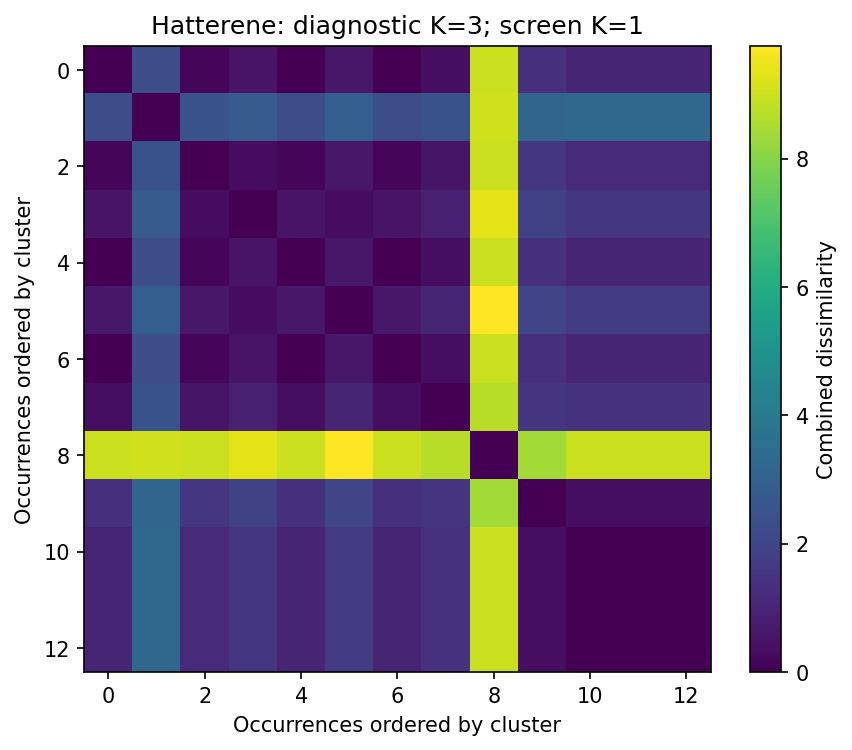
\includegraphics[width=\linewidth]{figures/hatterene-heatmap.png}\caption{Pairwise dissimilarity.}\end{subfigure}\hfill
\begin{subfigure}{.48\linewidth}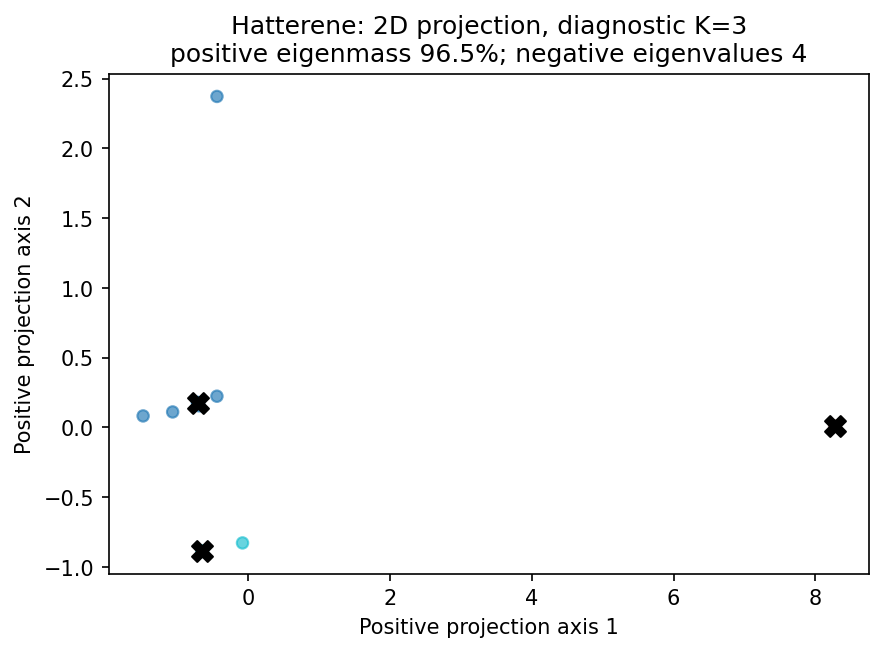
\includegraphics[width=\linewidth]{figures/hatterene-projection.png}\caption{Two-dimensional projection.}\end{subfigure}
\caption{Hatterene under SP+learned moveset dissimilarity, diagnostic $K=3$ (8/1/4), with selected $K=1$. In (a), every cell is a pairwise build dissimilarity; occurrences are ordered by the saved cluster labels and the color bar encodes magnitude. In (b), \projkey\ The visually isolated occurrence and the projection are small-sample diagnostics, not independent validation. Original figures are reproduced unchanged.}
\end{figure}
\end{landscape}
\clearpage

\subsection{Incineroar: primary comparison of two dissimilarities}
The 197-occurrence population is large enough to expose distinct neighborhoods but remains selectively published and source-dependent. The comparison below holds the occurrence set fixed and changes the dissimilarity. Cluster numbers are arbitrary within a model: SP-only cluster 0 and learned cluster 0 are not presumed to be the same group.

\begin{table}[!ht]\centering\small
\caption{Selected and diagnostic partitions from saved results. ARIs list all three limited group-subsample comparisons. A dash means silhouette is undefined at $K=1$, not zero.}
\resizebox{\linewidth}{!}{\CandidateTable}
\end{table}
SP-only selects $K=3$, with sizes 31/24/142 and silhouette 0.727. All three retained-anchor ARIs are 1.000 (158, 155 and 159 Incineroar anchors, respectively). This establishes stability under the current narrow procedure, not invariance across datasets or validated tactical labels.

For SP+learned movesets, the selected display is $K=1$. Its diagnostic $K=2$ split is 190/7, silhouette 0.838, with ARIs 1.000/0.282/$-0.010$. The high separation is partly a rare-package effect. Diagnostic $K=3$ has sizes 34/7/156, silhouette 0.545 and ARIs 1.000/0.759/0.765. The seven-member group fails the uniform size threshold of 20. Thus rejection by the screen and qualitative interest in that group are compatible conclusions.

\begin{table}[!ht]\centering\small
\caption{Occurrence overlap between the two saved Incineroar $K=3$ partitions. Rows use SP-only cluster indices; columns use learned-combined indices. This is a membership comparison, not a tactical confusion matrix.}
\CrossTable
\end{table}
The overlap shows which allocations remain together and which are regrouped after moveset differences enter. Subsequent pages pair the saved combined-distance figures with newly prepared SP-only counterparts. Only presentation projections were calculated from the stored matrices; no cluster assignments, scales, weights or medoids were refitted.
\clearpage

\subsubsection{What the combined-distance diagnostic partition contains}
The 34-occurrence group has Speed SP 11--32, relatively higher than the large group's 0--13 range. Its medoid is $30/0/1/0/12/23$, Careful, Intimidate and Sitrus Berry, with Fake Out / Flare Blitz / Parting Shot / Throat Chop. Calling it a relatively higher-Speed neighborhood is a description of investment, not an asserted exclusive tactical purpose.

The seven-occurrence group has Attack SP 31--32. All seven share the complete set Fake Out / Close Combat / Flare Blitz / Darkest Lariat. Items are Life Orb (4), White Herb (2) and Charcoal (1). Its medoid is $32/32/0/0/0/2$, Brave, Intimidate and Charcoal. These are seven genuine observations, not one unique build artificially multiplied by a deduplication correction. Their recurring package is interesting even though the group fails the same minimum-size threshold used for larger populations.

The 156-occurrence group is comparatively low-Speed and bulk-oriented; its medoid is $31/0/14/0/19/2$, Impish, Intimidate and Sitrus Berry, again with Fake Out / Flare Blitz / Parting Shot / Throat Chop. It includes several nonzero and even high-Attack configurations. The higher-Speed group also contains some Attack investment. Consequently the learned partition does not implement a simple attacker-versus-support dichotomy. Fake Out, a damaging move and Parting Shot can coexist in a real hybrid configuration.

\subsubsection{Separation depends on both model and representation}
SP-only separation is driven entirely by nonlinear investment differences. Its 24-occurrence cluster need not coincide with the seven same-moveset observations selected by the learned distance. Adding global move associations can distinguish a recurrent four-move package even when multiple original allocations occupy it; the small positive-median move scale can further emphasize that package. The resulting partitions answer different descriptive questions.

The three limited subsamples provide evidence that the SP-only partition is repeatable under source omission, but no independent external sample confirms it. Conversely, the seven-observation learned subgroup is coherent in its observed moveset but too rare to pass the uniform screen. A future rare-cluster analysis could investigate whether an alternative assessment is justified; the present report neither changes the screen nor promotes a rare group to a validated archetype.

\subsubsection{Reading the comparison figures}
Heatmap intensity encodes the actual matrix used by each model. Color bars have different units after normalization, so hue alone cannot compare absolute magnitudes across panels. Each heatmap is ordered by its own saved labels; corresponding row positions need not refer to the same occurrence. The overlap table, rather than visual row alignment, compares membership.

Projection colors refer to saved partitions in the original dissimilarity space. Classical MDS retains positive axes but cannot remove the distortion implied by negative eigenvalues. A visually dramatic gap can therefore coexist with limited stability or worse target reconstruction. SP boxplots summarize original observed allocations, not coordinates of the projection or fitted synthetic centroids. Cluster indices remain local to the respective model throughout.
\clearpage
\begin{landscape}
\begin{figure}[p]\centering
\begin{subfigure}{.48\linewidth}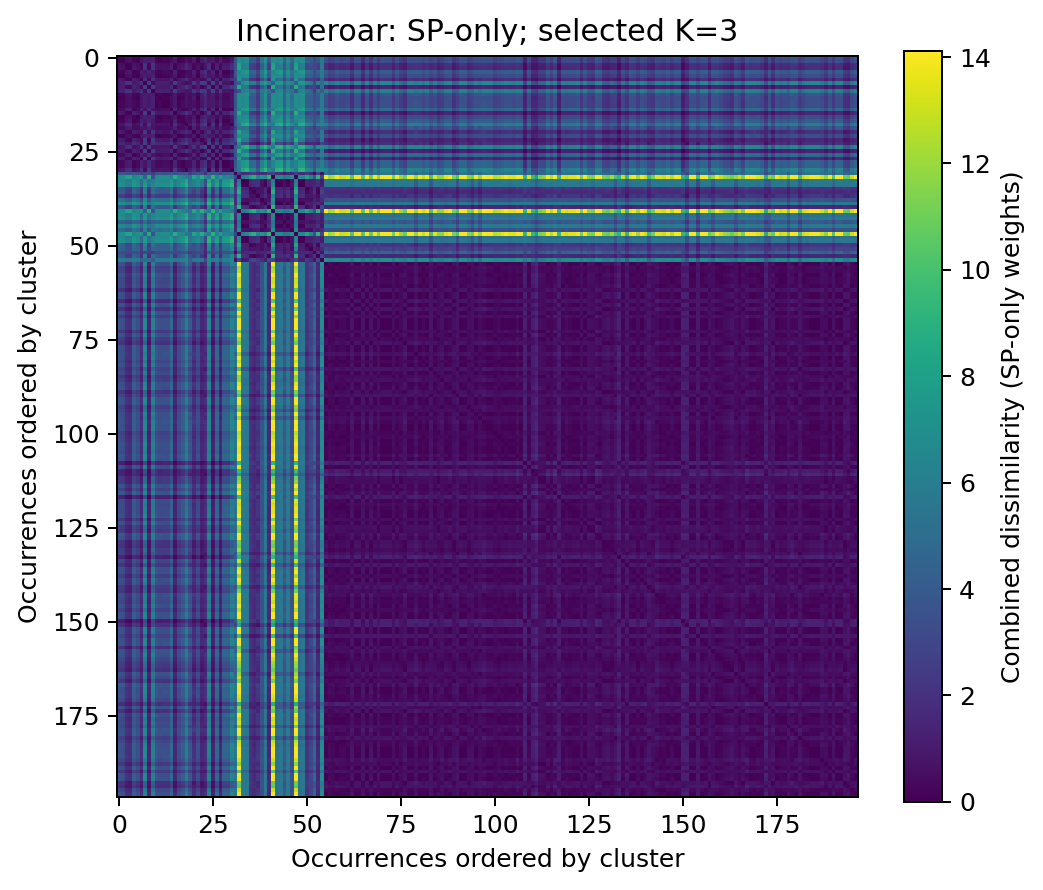
\includegraphics[width=\linewidth]{figures/incineroar-sp-only-heatmap.png}\caption{SP-only; selected $K=3$: 31/24/142.}\end{subfigure}\hfill
\begin{subfigure}{.48\linewidth}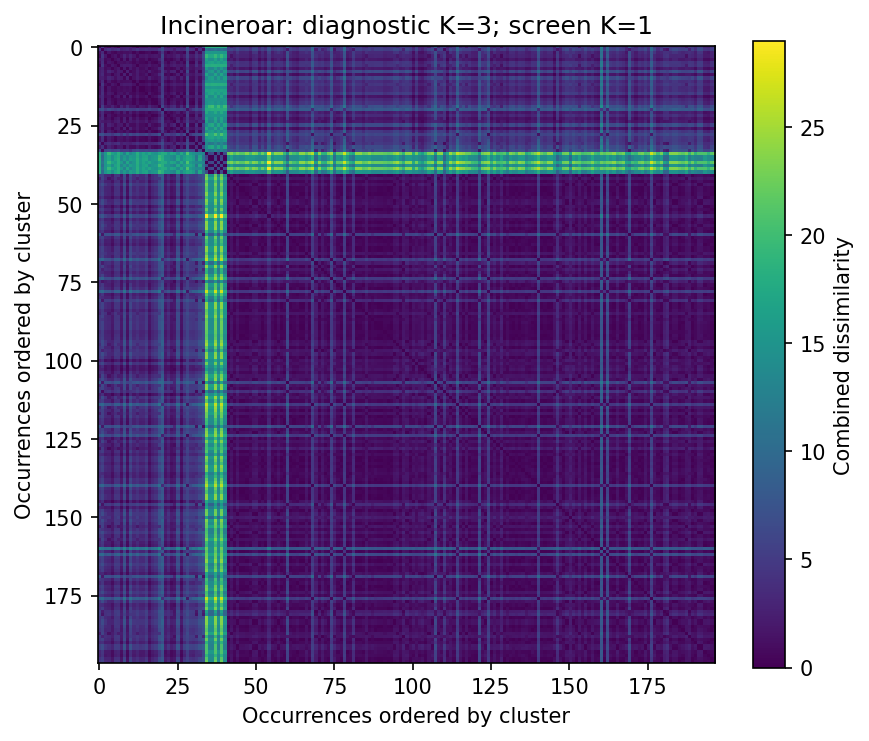
\includegraphics[width=\linewidth]{figures/incineroar-heatmap.png}\caption{SP+learned; diagnostic $K=3$: 34/7/156.}\end{subfigure}
\caption{Incineroar distance-structure comparison. Each cell is the pairwise build dissimilarity; occurrences are ordered by the corresponding saved cluster assignments. Color encodes dissimilarity magnitude, not a tactical class, and each panel has its own scale. Panel (a) is a new presentation plot of the saved SP-only matrix. Panel (b) is the existing combined-distance figure, copied unchanged; its conservative selected count is $K=1$. Different ordering means the same pixel position does not necessarily represent the same pair of occurrences.}
\end{figure}
\end{landscape}
\clearpage
\begin{landscape}
\begin{figure}[p]\centering
\begin{subfigure}{.48\linewidth}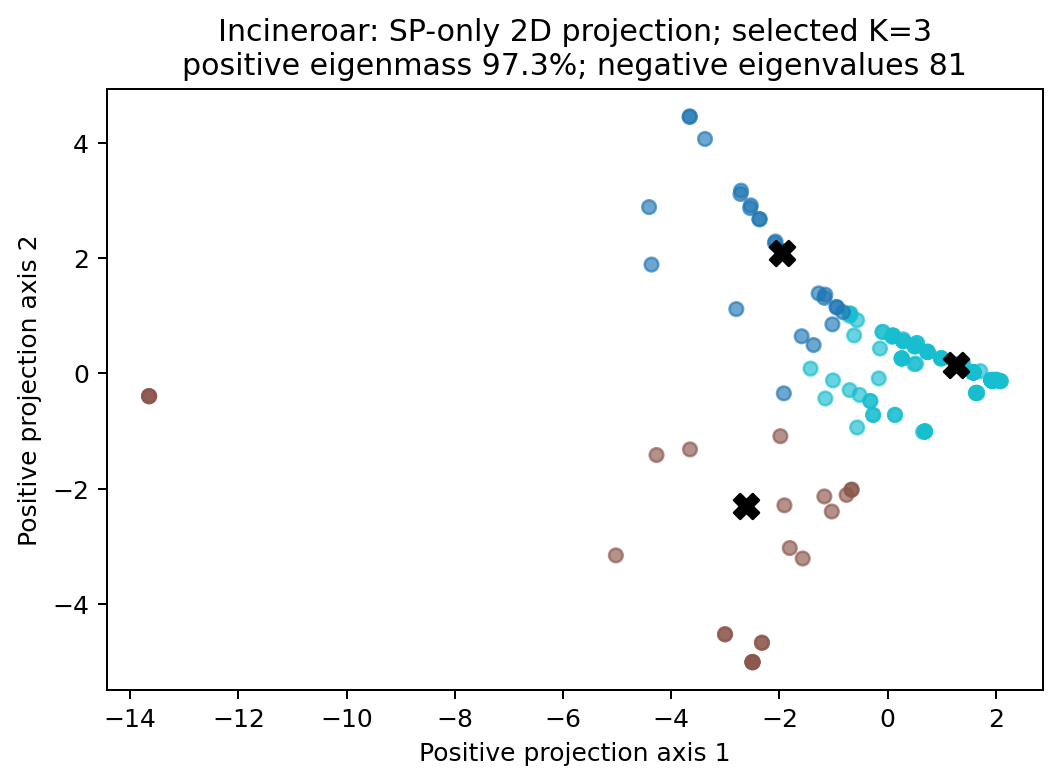
\includegraphics[width=\linewidth]{figures/incineroar-sp-only-projection.png}\caption{SP-only; selected $K=3$.}\end{subfigure}\hfill
\begin{subfigure}{.48\linewidth}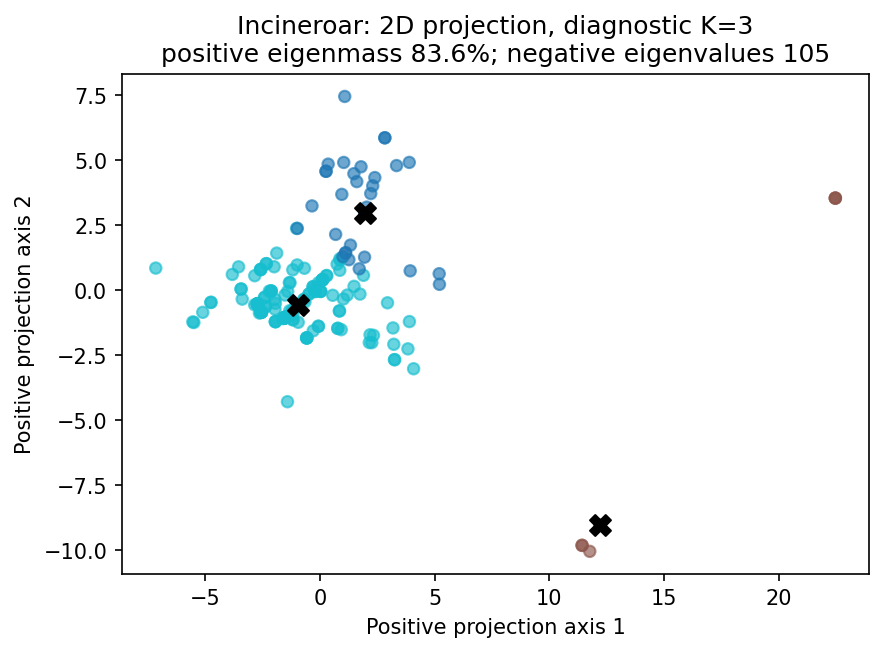
\includegraphics[width=\linewidth]{figures/incineroar-projection.png}\caption{SP+learned; diagnostic $K=3$, selected $K=1$.}\end{subfigure}
\caption{Incineroar neighborhood projections. \projkey\ The left panel uses the saved SP-only matrix and 31/24/142 labels; the right is the unchanged existing projection of the learned-combined matrix and 34/7/156 labels. No clustering was performed in either plotted coordinate system. The positions, orientations and color identities are model-specific; apparent gaps alone do not establish generalization or tactical meaning.}
\end{figure}
\end{landscape}
\clearpage
\begin{figure}[p]\centering
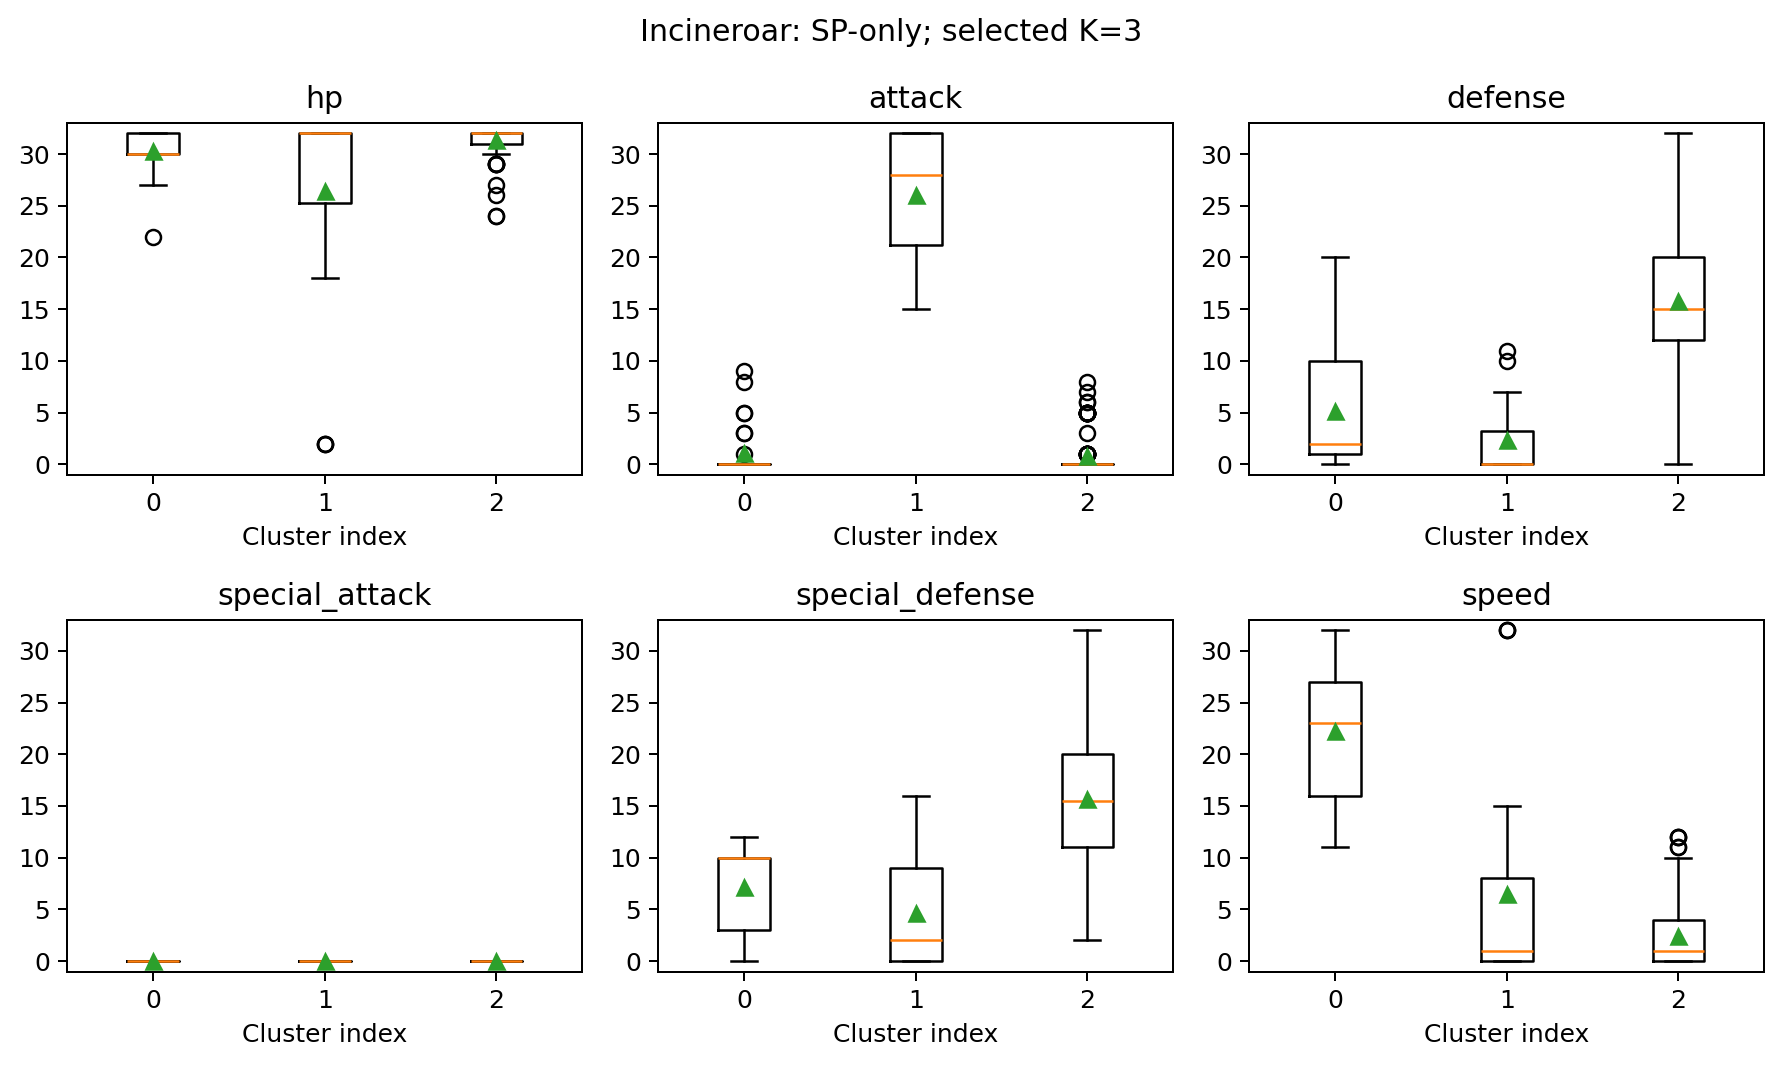
\includegraphics[width=.94\linewidth]{figures/incineroar-sp-only-boxplots.png}\\[3mm]
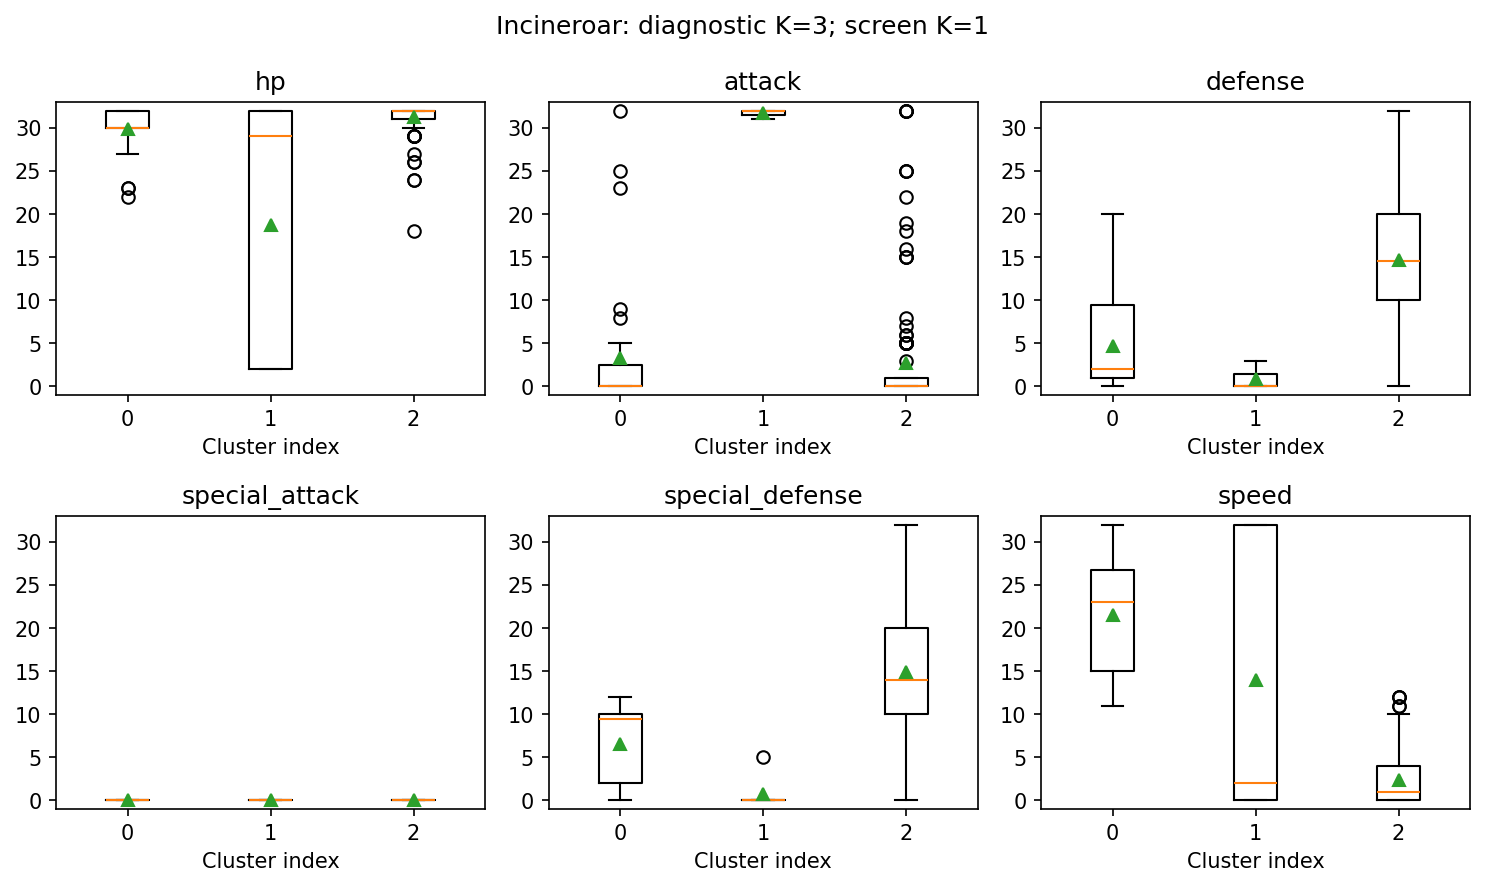
\includegraphics[width=.94\linewidth]{figures/incineroar-sp.png}
\caption{Incineroar original training allocations under two different partitions. Top: SP-only selected $K=3$ (31/24/142); bottom: existing SP+learned diagnostic $K=3$ (34/7/156), whose selected display remains $K=1$. Each panel's horizontal axis is its model's cluster index and its vertical axis is the indicated original SP value. \boxkey\ The bottom high-Attack group has seven occurrences, not the 24-member SP-only group. No fields have been averaged into new builds.}
\end{figure}
\clearpage

\subsection{Mega Raichu Y: a sensitive default split}
The 72 compatible observations have 53 distinct full configurations and 47 training cores. All have Attack SP 0 and the required Raichunite Y item. The population therefore cannot test discrimination among Attack-investment levels or meaningful item-identity prediction, even though the implementation supports those dimensions.

The SP-only screen retains $K=1$. With the default learned-combined distance it selects $K=2$, sizes 46/26, silhouette 0.442 and subsample ARIs 0.747/0.734/0.746. The first group spans Speed SP 9--28; the second spans 28--32. Their medoids are $30/0/12/0/0/24$ and $30/0/4/0/0/32$, respectively. The first source medoid has Protect / Zap Cannon / Fake Out / Focus Blast; the second has Zap Cannon / Encore / Fake Out / Focus Blast. The original ability assertion is preserved; compatibility with the active Mega context is checked separately by the established adapter.

At diagnostic $K=3$, a single Special Attack 32 observation is isolated. That extra singleton is not accepted as a recurring independent archetype. Higher separation under an additional cut would not by itself justify it. The selected default $K=2$ also changes under gamma, defensive weight or move-weight choices (Section~10), so the result is evidence of an investment/moveset neighborhood in this sample, not a fixed tactical taxonomy.
\figone{mega-raichu-y-sp.png}{.96}{Mega Raichu Y, default SP+learned dissimilarity, selected $K=2$ (46/26). Horizontal axes are cluster indices; vertical axes are original SP coordinates. \boxkey\ Constant Attack and other near-constant fields limit which hypotheses this sample can test. Original figure reproduced unchanged.}
\clearpage
\begin{landscape}
\begin{figure}[p]\centering
\begin{subfigure}{.48\linewidth}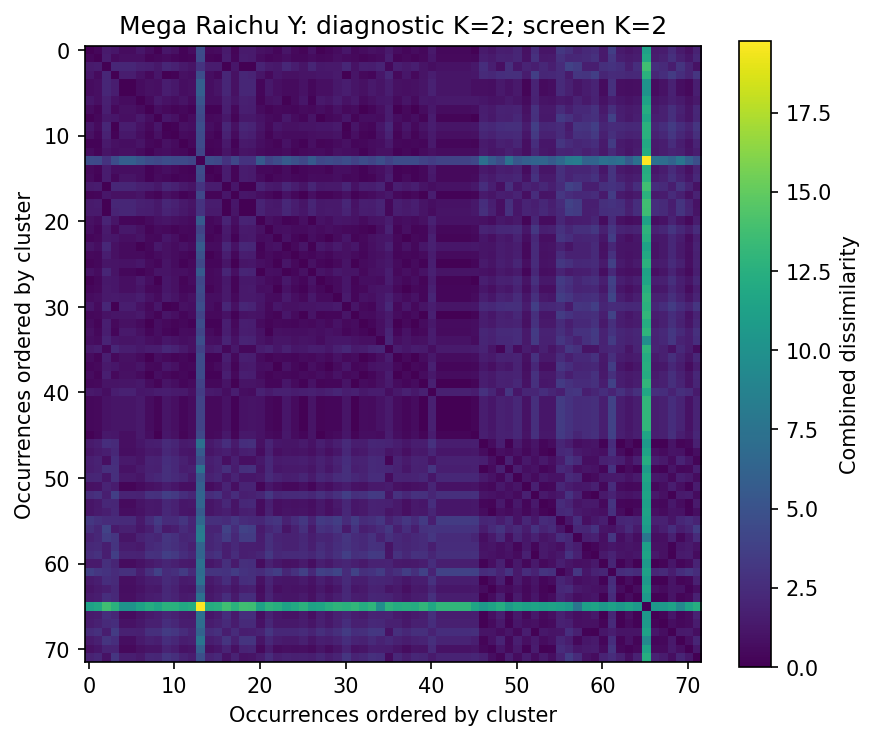
\includegraphics[width=\linewidth]{figures/mega-raichu-y-heatmap.png}\caption{Pairwise dissimilarity.}\end{subfigure}\hfill
\begin{subfigure}{.48\linewidth}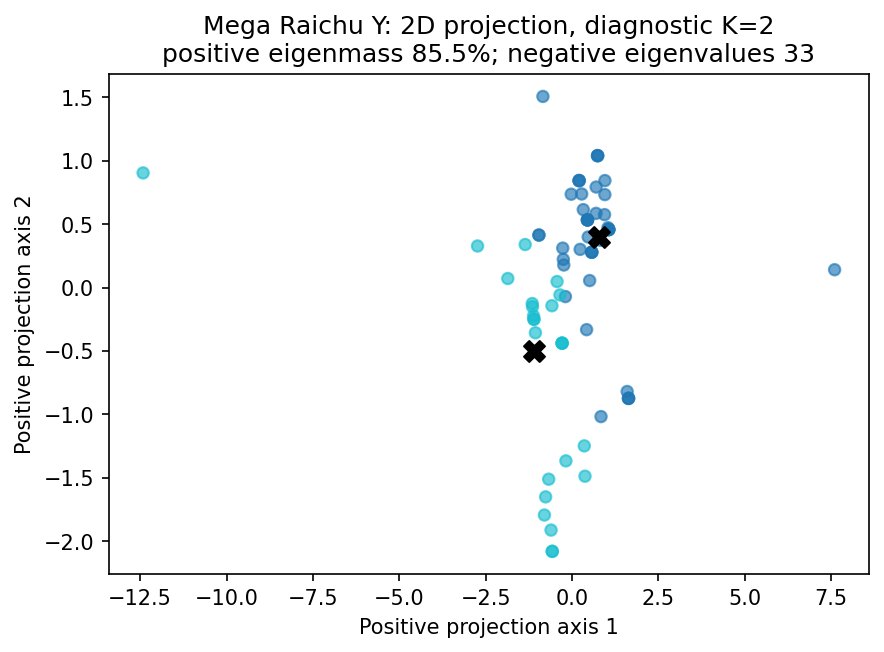
\includegraphics[width=\linewidth]{figures/mega-raichu-y-projection.png}\caption{Two-dimensional projection.}\end{subfigure}
\caption{Mega Raichu Y, default learned-combined dissimilarity, selected $K=2$ (46/26). Every heatmap cell is a pairwise build dissimilarity, with occurrences ordered by the saved clusters and magnitude encoded by the color bar. In the projection, \projkey\ SP-only selected $K=1$ is a separate result and is not depicted here. Both existing figures are copied unchanged.}
\end{figure}
\end{landscape}
\clearpage

\section{Grouped, target-masked held-out evaluation}
The evaluation uses three deterministic hash folds at the connected source/team level. Embedding vocabulary, frequencies, association/SVD, species normalization and train medoids are fitted only on training occurrences. Evaluation builds are transformed without refitting; the saved split audit retains training IDs, group membership, neighbors and predictions. Source grouping protects against known related records but does not establish fully independent samples.

For each target, five nearest training occurrences predict the target by a median for numeric SP or majority vote for canonical item identity. The comparator is the species-specific training median or mode. Speed, Attack and Special Attack targets remove their respective SP terms before scale fitting and neighbor search. Bulk prediction removes all HP/Defense/Special Defense terms. Item prediction removes item mismatch. Other observed coordinates and optional nature remain covariates; final calculated stats are not included. This is conditional reconstruction from the remaining known attributes, not prediction from the sparse evidence available in an actual battle.

\begin{table}[!ht]\centering\small
\caption{Three-fold grouped holdout errors. Numeric columns are mean absolute errors in SP units; the last column is a categorical item-identity error rate, not an SP error. Every method evaluates 13 Hatterene (13 groups), 197 Incineroar (192 groups) and 72 Raichu Y (70 groups) occurrences.}
\resizebox{\linewidth}{!}{\HoldoutTable}
\end{table}
Learning move association does not improve any tested numeric target over SP-only in these populations. For Incineroar, SP-only Speed MAE is 1.421, compared with 2.142 for Jaccard and 2.898 for learned association; the corresponding bulk errors are 1.320, 2.076 and 2.832. Both move-based variants can outperform the global-median baseline while still underperforming the simpler SP neighborhood.

Incineroar item error is 0.305 with learned association versus 0.381 with SP-only and 0.310 with the training mode. The small improvement over the mode is exploratory, without a confidence interval or external replication. Hatterene's methods tie on this sample. Constant Attack and item in Raichu Y, and constant Special Attack in Incineroar, make zero error uninformative about learning. Three folds and three stability subsamples do not justify a claim of broad generalization or calibrated uncertainty.
\clearpage

\section{Discussion: useful structure without a validated taxonomy}
\subsection{What the study establishes}
Nonlinear investment differences provide interpretable neighborhoods without averaging illegal joint builds. SP-only Incineroar has a repeatable partition under the current limited source-group omission procedure; Hatterene reveals defensive variation around a nearly constant offensive core. Learned moveset association identifies a recurring high-Attack Incineroar package. These are concrete structures in observed records, not merely hypothetical roles chosen before fitting.

A rare coherent variant can be scientifically interesting even when a uniform minimum-size threshold rejects it. Seven source occurrences sharing a four-move package deserve inspection; the rejection states that the current acceptance rule does not support selecting the whole partition. It does not state that the observations are noise or that their tactical intent has been established. Conversely, a stable or visually separated cluster is not automatically useful for reconstructing masked attributes.

\subsection{Normalization and hyperparameter sensitivity}
\begin{table}[!ht]\centering\small
\caption{Conservative selected $K$ under the fixed sensitivity grid. The entries describe the saved screen, not an optimization outcome. ``Proportion'' replaces the defensive decomposition; dimension settings change only the retained SVD dimensions.}
\SensitivityTable
\end{table}
Raichu Y's selected count changes from 1 to 2 or 3 across nearby settings. Incineroar's default learned count remains one, while reducing the move weight permits a three-cluster screen result. The alternative proportional-bulk distance likewise does not yield a universally better partition. These changes demonstrate that ``number of archetypes'' is partly a modeling decision, not a direct data label. Positive-median scaling may amplify a rare moveset difference; robust scaling should be investigated rather than tuned post hoc until a preferred role narrative emerges.

Global move associations may also encode species prevalence and complementary packages. Mean pooling loses interactions, while rarity shrinkage cannot create missing evidence. A future evaluation should distinguish genuine move substitution from co-use and assess predictive utility under realistic partial battle observations. The present heldout tasks do not resolve that issue.
\clearpage

\section{Future research questions}
Future work should begin with evaluation design rather than immediate battle integration. Which SP penalties preserve useful neighborhoods across held-out source populations? Can sensitivity scales or defensive-allocation weights be selected on a separate development sample without overfitting a tiny species population? Amount/proportion decomposition avoids some double-counting but may discard important allocation information near zero bulk; alternative penalties need explicit mathematical and empirical comparison.

A second question concerns the learned-move scale. A quantile-based or capped normalization might reduce the leverage of rare differences, but any change should be evaluated against SP-only and exact overlap on untouched groups. More realistic move-set representations could retain pair interactions or distinguish complementary moves from substitutes. Their added complexity would require demonstrable benefit beyond more attractive projections.

Rare-cluster assessment also needs a defensible objective. A uniform size threshold rejects a small coherent package; relaxing that threshold solely because a subgroup looks meaningful would introduce analyst bias. Appropriate future work could compare stability across genuinely independent sources, distinct training cores and frequencies, while preserving original occurrence weights and reporting the uncertainty of small groups.

Masked-observation assignment is another open problem. The current distances compare complete builds, whereas battle evidence is partial and time-dependent. Distances to medoids or similarity memberships must be defined without filling unknown SP, moves or items with arbitrary defaults. The same revealed move must not be counted twice, once as a deterministic constraint and again as an independent probabilistic observation.

Finally, clustering-based, nearest-neighbor and kernel-based priors could be compared over legal \emph{joint} configurations. Such work would need a principled treatment of unseen configurations, source selection, conditional normalization and hard evidence. A marginal distribution for each stat would not preserve the shared SP budget, nature alignment, item correlation or team matching relation. Eventually the useful outputs may be distributions of action-time Speed order and potential damage, but those distributions require verified mechanics and calibration. None of these priors, synthetic samplers, posterior models or strategy recommendations is implemented in this milestone.

\section{Conclusion}
The project now distinguishes evidence-backed feasible configurations from descriptive published usage, and has an offline framework for examining similarities among real complete builds. The experiments preserve source multiplicity, expose nonmetric distance choices, retain observed medoids and evaluate training-only representations under grouped target masking. They establish a reproducible foundation for studying build archetypes.

The findings are mixed. Hatterene does not support a selected multi-cluster interpretation; Incineroar's SP-only structure is clearer under the current screen than its learned-combined structure; and Raichu Y's default split is sensitive to nearby choices. A small coherent Incineroar moveset neighborhood is worth examining, but learned association does not improve numeric target prediction over SP-only. These results support continued comparative research, not a claim that universal tactical roles or calibrated hidden-build probabilities have been discovered. This reporting milestone stops for human review.
\clearpage

\section*{Reproducibility, provenance and research status}
\addcontentsline{toc}{section}{Reproducibility and sources}
The primary numerical artifact is the completed M3.5.1 run identified by \texttt{7933afbb341cdbeddbe3}, referenced by \path{.cache/research/m351/latest.json}. Its directory contains the 47-stage manifest, \texttt{population.json}, species/configuration JSON, \texttt{moves.json}, stability results and \texttt{heldout.json}. Matrix rows and assignments retain immutable occurrence IDs. The full local matrices are deliberately not distributed as document assets.

This report includes a compact \texttt{evidence-summary.json} with exact source hashes, selected medoids' complete original configurations and provenance, saved metrics and figure provenance. It also bundles every used figure: eleven original PNGs copied byte-for-byte and three new SP-only Incineroar presentation plots. The new heatmap and boxplots use saved assignments; classical MDS is calculated only to visualize the saved matrix. No clustering, source collection, OCR, inference or damage calculation was rerun for M3.5.2.

\texttt{report.tex}, \texttt{results\_tables.tex}, the figures directory and \texttt{build.sh} suffice to regenerate the PDF with a normal LaTeX installation. The optional \texttt{prepare\_report.py} refreshes presentation assets from the preserved local study, without importing the inference or clustering implementation. Package versions, checks and archive policy are documented in the accompanying README. Rendering validation checks page contents, figure hashes, references and representative visual pages; it does not imply independent scientific acceptance.

Earlier mechanics evidence is source-specific. Official rule documentation supports the item-clause scope recorded in R5; 52Pok\'e provides pinned Champions stat and contextual mechanics descriptions; canonical local data supplies identities; executable Showdown/calculator references supply conditional numerical behavior. No source is authoritative for every field. A Generation 9 learnset is not substituted for Champions availability, and observed co-occurrence does not establish learnability, equipped slots or move probabilities. Unresolved mechanics remain unresolved. The source-reviewed Battle 12 ownership envelope and independent human acceptance are still limitations.

\subsection*{Sources and local research artifacts}
\begin{enumerate}[label={[R\arabic*]}]
\item \textbf{Joint stat feasibility.} \path{reports/M3.1.2-champions-stat-feasibility.md}, 15 October 2026. Exact joint-budget representation and stat-domain gaps. Pinned source metadata: \path{knowledge/data/champions_stat_rules.json}. 52Pok\'e contributors, \emph{Stats} revision 2607357; \emph{Nature} revision 2568467; \emph{Pok\'emon Champions} revision 2628728, retrieved 15 October 2026. Community documentation with recorded CC BY-NC-SA 3.0 attribution, not official mechanics certification.
\item \textbf{Causal Speed case study.} \path{docs/m3.2.2-battle11-speed-report.md}. Historical Battle 11 evidence-linked order constraints and support reduction. Its older eligibility counts are historical and are not substituted for the M3.5.1 data population.
\item \textbf{Damage inference and attribution.} \path{reports/M3.4.2-offensive-stat-inference.md} and \path{reports/M3.4.3a-hatterene-damage.md}, October 2026. Pinned \texttt{@smogon/calc 0.12.0} Champions generation-0 reference, commit \texttt{9c57e9b8c1d8a7403b71c10042136ea5e001593b}; conditional integer calculations and unresolved coverage.
\item \textbf{Empirical occurrences and soft moves.} \path{reports/M3.4.4-soft-move-evidence.md}. Full occurrence-preserving selection, source templates and the fixed $\alpha=0.5$ scoring experiment. Original external data: vgcmulticalc tournament-published VGC M-C Doubles exports, with per-occurrence source URLs preserved in local artifacts.
\item \textbf{Latest reviewed item/ownership state.} \path{reports/M3.4.5a-team-items-and-stat-review.md}, 23 October 2026; fixtures \path{battle12-m344-damage-review.json} and \path{battle12-m345a-team-item-review.json} under \path{tests/fixtures/battle_evidence/}. Team rule metadata: \path{battle_evidence/data/team-item-rule-v1.json}. This later ownership analysis supersedes simpler original-owner assumptions; independent human acceptance remains open.
\item \textbf{Maintained stat implementation.} \path{knowledge/champions_stats.py} and the source-specific stat metadata in R1. Base-stat identity is supplied by the existing KnowledgeBase, not a new database or a report-specific approximation.
\item \textbf{Primary offline experiment.} \path{reports/M3.5.1-build-similarity.md}, \path{reports/M3.5.1-validation.md}, and completed local study fingerprint \texttt{7933afbb341cdbeddbe3}, 24 October 2026. 129 recorded portable checks passed, three historical-artifact cases deselected; those are prior experiment checks, not a new recognition benchmark.
\end{enumerate}
\end{document}
